\documentclass{bioinfo}
\copyrightyear{2014}
\pubyear{2014}
\usepackage{xspace}
\newcommand{\ps}{phylesystem\xspace}
\newcommand{\otol}{Open Tree of Life\xspace}
\newcommand{\nexson}{otNexSON\xspace}
\newcommand{\js}{JavaScript\xspace}
\newcommand{\mthcomment}[1]{{\color{red} \textsc{#1}}\xspace}
\newcommand{\ejmcomment}[1]{{\color{green} \textsc{#1}}\xspace}
\newcommand{\jfacomment}[1]{{\color{blue} \textsc{#1}}\xspace}

\usepackage{natbib}
\bibliographystyle{apalike}

\usepackage{hyperref}
\hypersetup{colorlinks=true, linkcolor=black, citecolor=black, hyperindex=true, backref}
\begin{document}
\firstpage{1}
\title[phylesystem git phylostore]{Phylesystem: a git-based data store for community curated phylogenetic estimates}

\author[McTavish\textit{et~al}]{
    Emily Jane McTavish,$^{1,2}$
    Cody E.~Hinchliff,${^3}$
    James F.~Allman,${^4}$
    Joseph W.~Brown,${^3}$
    Karen A.~Cranston,${^5}$
    Mark T.~Holder,$^{1,2}$\footnote{to whom correspondence should be addressed}~
    Jonathan A.~Rees,${^5}$
    Stephen Andrew Smith${^3}$
}
\address{$^{1}$Department of Ecology and Evolutionary Biology, University of Kansas, Lawrence KS, USA\\
$^{2}$Heidelberg Institute of Theoretical Studies, Heidelberg, Germany \\
$^{3}$Department of Ecology and Evolutionary Biology, University of Michigan, Ann Arbor, Michigan, USA\\
$^{4}$Interrobang Corporation, Wake Forest, North Carolina, USA\\
$^{5}$National Evolutionary Synthesis Center, Duke University, Durham, North Carolina, USA}
\history{Received on XXXXX; revised on XXXXX; accepted on XXXXX}

\editor{Associate Editor: XXXXXXX}

\maketitle

\begin{abstract}
\section{Motivation:}
Archival storage of phylogenetic estimates from published studies can be accomplished
    using general platforms like Dryad \citep{Dryad} or TreeBASE \citep{SandersonDPE1994}.
Those services fulfill a crucial role in making phylogenetic studies be more transparent
    and reproducible.
However, available trees nearly always require some editing to improve the accuracy and reusability of the phylogenetic statements.
Many trees in data archives or supplemental files from publications are incorrectly rooted.
Establishing the linkage between tip labels used in a tree and taxa in a single taxonomy 
    dramatically improves the ability of other researchers to reuse phylogenetic estimates.
Because the process of curating a published phylogenetic estimate is not error-free,
    retaining a full record of the provenance of edits to a tree is crucial for
    openness, allowing editors to receive credit for their work, and
    making errors introduced during curation easier to correct.

\section{Results:}
Here we report the development of software infrastructure to support the open curation of
    phylogenetic data by the community of biologists.
The backend of the system provides an interface for the standard database operations of
    creating, reading, updating, and deleting records by making commits to a git repository.
The record of the history of edits to a tree is preserved by git's version control features.
Hosting this datastore on GitHub provides a open access to the data store using tools
    familiar to many developers.
We have deployed a server running the ``phylesystem-api'', which wraps the interactions with git and GitHub.
The \otol project has also developed and deployed a \js application that uses the \ps-api and
    other web services to enable input and curation of published phylogenetic statements
\section{Availability:}
Source code for the web-service layer is available at \url{https://github.com/OpenTreeOfLife/phylesystem-api}.\\
%The library \url{https://github.com/OpenTreeOfLife/peyotl} is a prerequisite.
The data store can be cloned from: 
\url{https://github.com/OpenTreeOfLife/phylesystem}.
A web application that uses the \ps web services is deployed
at \url{http://tree.opentreeoflife.org/curator}.
Code for that tool is available from 
\url{https://github.com/OpenTreeOfLife/opentree}.

\section{Contact:} \href{mailto:mtholder@gmail.com}{mtholder@gmail.com}

\end{abstract}

\section{Introduction}

Characterizing and systematizing relationships among species has been a goal of biologists since Linnaeus \cite{Linne1758}.
The phylogenetic systematics ``revolution'' of the 1960's focused most of the effort toward this goal on the 
    task of estimating phylogenetic relationships.
The rapid growth in availability of molecular data, the development of models and software implementations for
    inferring phylogenies and the appreciation of the importance of phylogenetically-aware comparative methods
    \citep[e.g.][]{Felsenstein1985Comp} have led to dramatic increases in the number phylogenetic estimates.


Unfortunately, capturing the inputs and outputs of a phylogenetic analysis in a rich, standardized form is
    wide range of inputs and making few or no
    guarantees to users of the database that the records will be in any particular form.
This encourages sharing of data by making the submission process fast and easy, and is advantageous under Dryad's
    general purpose archival model--Dryad's scope is not limited to phylogenetic information.
However, if the authors submitting the data are not conscientious in their explanations of the data, it can be difficult
    for users of the data to reliably extract all of the necessary information from the archive, or the data may not contain sufficient metadata for reuse.

On the opposite end of the spectrum, some databases require data providers to conform to rigorous
    standards with respect to input format and content.
Since 1994, TreeBASE \citep{SandersonDPE1994} and its successor TreeBASE version 2 \citep{TreeBase2} have served
    as the primary archival data stores for phylogenetic estimates and the data that these trees are based on.
As of 2014, TreeBASE contains 4076 studies and over 12,800 trees \citep{TreeBaseWebCite}.
Many journals encourage or require that each publication that estimates phylogenetic trees cite a TreeBASE
    deposition containing the associated trees.
TreeBASE produces a much more feature-rich interface for phylogenetic queries than Dryad, because each 
    TreeBASE submission is parsed thoroughly and converted to a set of records in a relational database.
The downside of this approach is that it requires that submissions correspond to a more uniform format and without constant updating,
    that format may not reflect new types phylogenetic data being generated.

Unfortunately, file formats read and written by tree estimation tools are idiosyncratic and often so 
    terse that they omit useful information about the analysis (see \citet{StoltzfusEtAl2012} for a discussion
    of this topic and other challenges relating to the archiving of phylogenetic estimates).
As a result, the TreeBASE submission process usually requires the authors of a data package to reformat their data, correct
    the rooting of the tree, alter the labels of the tips of the tree, {\em etc}.
The TreeBASE project provides a 12-minute video 
    \footnote{\url{http://treebase.org/treebase-web/submitTutorial.html}} 
    explaining the non-trivial procedure of preparing a submission.
Because these steps are often taken after the analyses for a publication are complete, it is more likely 
    errors introduced in the submission process will not be corrected until an observant user tries to reuse the data.
If there were a universally used, rich file format for phylogenetics analyses, then import constraints such as those
    used by TreeBASE would be less of a hurdle, since the critical metadata regarding rooting, labels, etc. could be
    stored alongside the tree itself.
The xml-based NexML specification \citep{NeXML} defines such a format, but it is not widely used by tree estimation tools.
We hope to overcome some historical problems with adoption of rich file formats for phylogenetics 
   by providing tools for easily curating data and converting among formats.

Thus, the current state of phyloinformatic archival infrastructure is ripe for improvement in numerous ways.
One such opportunity is the development of a datastore that allows the community of biologists to improve the
    accuracy and re-usability of published phylogenetic statements.
We describe here an implementation of one such system, which we call ``phylesystem'' because it uses a set of
    versioned text files on the filesystem (and the fact that we {\em love} bad puns).
The goal of \ps is not to replace systems like Dryad or TreeBASE, but to complement them by 
    storing phylogenetic statements and associated metadata in a consistent format while retaining the history of
    edits that were made to the data themselves.
We anticipate that most of the trees stored in \ps will be associated with permanent, static archives
    elsewhere (usually either TreeBASE or Dryad).


\subsection{Approach}
One of the motivations of the design of \ps was to support the \otol's need for a curated set
    of rooted trees that have been aligned to a common taxonomy.
Additionally, one of the goals of the \otol project was to support infrastructure for phylogenetic
    research in an open way that encourages the community of biologists to participate in the 
    collection and curation of our knowledge of the phylogenetic relationships of life on Earth.

Thus, our goals when designing \ps were to build: 
\begin{enumerate}
    \item  a data store capable of:
        \begin{enumerate}
            \item \label{fewKStudies} storing trees from thousands of published studies. We do not intend to store the 
                data upon which the phylogenetic estimates were based.
            \item \label{fewTreesPerStudy} storing a few exemplar trees from each study. We do not anticipate that the system will be used 
                to store thousands of trees from 
                an individual study (such as each sampled tree from a bootstrap or MCMC analysis, for example).
            \item \label{richAnnot} handling rich annotation of the trees, the taxa to which they refer to, and metadata describing 
                the analysis that produced the trees.
            \item \label{history} storing the full history of changes made to a study and its trees,
                including an identifier to indicate who made the changes.
        \end{enumerate}
    \item \label{ws} web services around the data store to support a user-friendly curation application run in the user's browser. These include services for validation of the files against a published schema.
    \item \label{looseOpen} a loosely coupled system that would allow the community of biologists to interact with the data in a wide variety of ways.
\end{enumerate}
From these requirements, we chose to implement \ps as a set of software wrappers around a data store
    which consists of a git \citep{git} repository of phylogenetic statements serialized as a \js Object Notation (JSON).
The data model used for the JSON is a close derivative of the NeXML standard for data interoperability \citep{NeXML},
  and can be converted back and forth using the peyotl library.

Our expectations that the system would have to store limited amounts of data for each study 
    (points \#\ref{fewKStudies} and \ref{fewTreesPerStudy} above) and that most
    studies would require relatively few edits imply that
    raw performance of the basic database operations was unlikely to be a bottleneck for most
    uses of the \ps.
This made it feasible to use text files as the format of the data store.
Thus far, in the six months since deployment of the study curation interface, the mean number of edits 
    per study is only 2.7. \ejmcomment{I'm checking I calculated this right. - this includes commits on studies that are no longer in the repo. Seems fine tho.}
The total size of the stored data (in JSON format with a line ending after 
    every field) is only around 150MB.

The requirement (\#\ref{history}, above) of maintaining a history of changes 
    (including an identifier for the editor) fits naturally with software version control systems.
We note that wiki engines such as Gollum use git version control as a backend database.
The idea of using git as general database has been discussed by others \citep{git-nosql-db}.

The requirement (\#\ref{richAnnot} above) to support rich annotations,
    is met by the NeXML data standard 
    This standard was designed
    to allow arbitrarily complex annotations of the entities that are crucial to phylogenetic statements.
Because \ps does not store character data, the entities included are the operational taxonomic units (OTUs), trees, nodes, and edges.

We opted to version JSON files to make it more efficient for the server to provide data for a client-side
    curation application that is written in \js (requirement \#\ref{ws} above).
We developed some syntactic conventions for converting XML to JSON tersely (described below as \nexson v1.0 and v1.2).
The adoption of these conventions reduced the web-service data payload size by approximately 50\% relative to 
    naive representation of NeXML in JSON.
This made it more feasible to load each study into the memory of the client's browser.
Despite the departure from the NeXML syntax, the \ps maintains the ability to export and ingest NeXML files.
Fundamentally the data model of the system is the data model of NeXML.

The final requirement (\#\ref{looseOpen}) of producing a maximally open,
    loosely coupled system is consistent with the use of a distributed
    version control system; git is the most popular distributed version control system.
Distributed version control systems do not require a single, ``primary'' repository.
Each copy of the repository maintains a copy of the entire history, and sharing documents between
    repositories is a peer-to-peer interaction.

Most people will probably think of the copy of the \ps repository that is listed under the \otol organization on
    the GitHub website (and stored on the GitHub servers) as the canonical version of the data store.
Indeed, this is likely to be the most easily accessible and highest profile clone of the \ps repo.
Nevertheless, other users of git are free to fork that repo and maintain their own variants of the data store.
Any such clone of the \ps repository maintains the ability to pull in changes from biologists who contribute
    edits to the \otol organization clone (for example, via \otol web applications).

The \otol project placed all of the code for the \ps under permissive, BSD-style licenses and the
    project makes no claim of ownership to any of the data in the repository. 
For new files deposited through the web application, the interface strongly encourages application of a CC0 copyright waiver, 
    allowing for later deposition in Dryad. Other data, including those files that originate from TreeBASE,
    do not have an explicit data license (although we believe that copyright does not apply to any of the data).

In most database-driven web services, the group of core maintainers who have shell access and 
    database passwords are the only people who have full access to the data in a data store.
Posting frequent dumps of a database can allow other users to obtain local copies of the data 
    for expensive, {\em ad hoc} calculations.
However, a local version of the data is clearly a second-class instance and the maintainers of the 
    canonical version of the database have {\em de facto} ownership of the project.
We hope that adopting a truly distributed backend for the datastore will reinforce the goals
    of the \otol project to build tools that can be used and controlled by the entire community of biologists 
    (rather than a few claiming ownership on the data store in perpetuity).

Currently the \ps web services use GitHub authentication for ``curators'' who edit studies.
The requirement that editors authenticate allows the provenance of each edit to include 
    a user name for the curator, while the use of GitHub credentials allows the \otol project
    to circumvent the need to maintain a database of users and passwords (or hashes).
Thus, there is no private database that would be required for someone to fork and maintain their
    own version of the corpus (on GitHub or elsewhere).
In future pull requests from forks of the \ps repo could contribute data to the main repository,
   but in order to maintain data quality at this time the phylesystem API (typically via the curation webapp) is the only method to add studies to the database.
The only private information relevant to \ps that is kept by the \otol project are the ssh-private
    keys that allow the project's web servers to push updated data to the GitHub-hosted clone of the 
    repository.

\begin{figure}
\caption{Workflow diagram} 
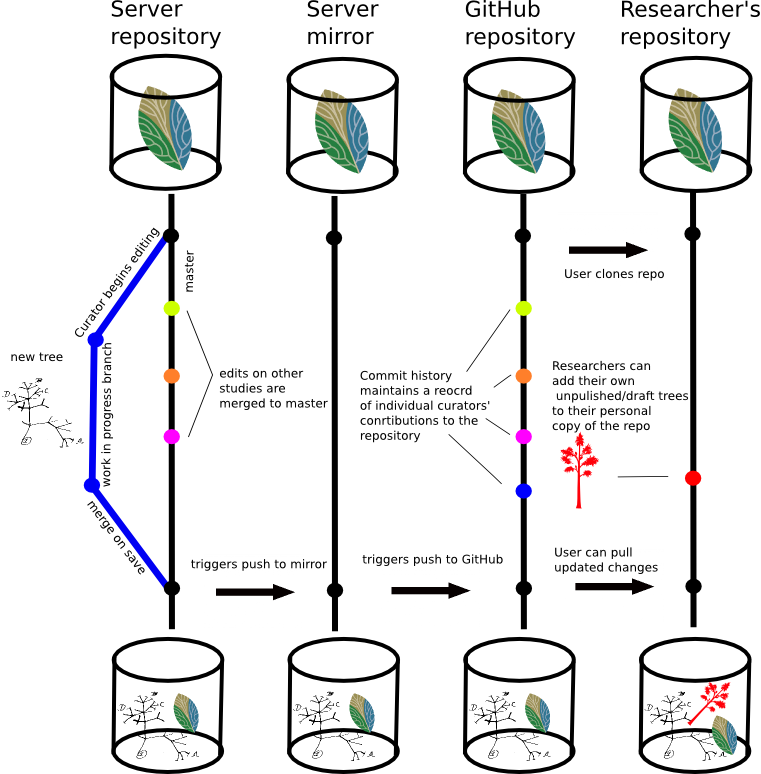
\includegraphics[scale=0.4]{workflow.png}
\label{workflow}
\end{figure}

\begin{methods}
\section{Methods}
The basic workflow of a curation session is:
\begin{enumerate}
    \item \label{loadAppStep} The user loads the curation webpage in his/her browser.  This fetches the \js curator application into the web browser.
    \item \label{otiListStep} A list of studies in the \ps is loaded from information in a study indexing service (called ``OTI'', see below).
    \item The user selects the study he/she would like to view.
    \item \label{getStudyStep} The curator application requests the study in \nexson form from the \ps server.
        The curator application also receives the git commit SHA (a checksum of the content ) of the repository at this point.
    \item \label{browseStep} The user may browse the studies and download representations of the data in NeXML, \nexson, NEXUS\cite{NEXUS}, or Newick formats without logging in.
    \item \label{authStep} If the user wants to edit a study, he/she must have a GitHub account (which are available free of charge) and must authenticate at this point.
    \item \label{userEditStep} The curator may correct tip taxon assignments with the help of taxonomic name resolution services (the ``taxomachine'' web services, which are described
        elsewhere) or fix the rooting information about the tree. The data model of the study is modified in the memory space of the 
        browser and maintained there until the curator chooses to save the study.
    \item \label{putStep} To save, the curator application uses an http PUT verb and includes the data (in \nexson), the starting SHA, and a commit message to support sensible history. 
        \ejmcomment{Do http verbs need more explanation somewhere?} 
        \jfacomment{It does seem to raise the topic of RESTful style. Not sure this is this relevant here.}
    \item \label{validateStep} The \ps-api code validates the \nexson (rejecting the request if the data is not a legal \nexson document).
    \item \label{gitSaveStep} If the data is a legal \nexson document, then a new git commit is created with the SHA
        provided in the PUT request as the parent commit. The commit is placed on a 
        ``work-in-progress'' branch in the git history to assure that the data is stored with 
        no chance of conflict.
    \item \label{gitMergeStep} If the study in question has not changed in the master branch 
        since the parent SHA, then the edit can safely be merged to the master branch.
        If this is the case, the merge is done and the work-in-progress branch is deleted.
        If the version of the study on the master branch {\em has} changed (e.g. if two users are simultaneously editing the same study),
        then the merge is not done. The data will be saved on the server, but not merged into the master branch.
        If the commit is not merged, then the merge must be later manually completed by a curator, as there is the potential for conflicts between changes made by different simultaneous edits.
    \item\label{gitTriggerPushStep}  If the new edit was successfully merged, then an event is triggered to tell the server to push the new master branch changes to the GitHub version
        of the repository.
    \item\label{respondStep} A response is returned to the curation app indicating whether or not the data was 
        merged to the master branch and including the new SHA that will serve as the parent for a future commit.
    \item\label{pushStep}  If the push event was triggered in step \#\ref{gitTriggerPushStep}, the updated master branch will be pushed to GitHub.
    \item\label{webHookStep} Using GitHub webhooks as a callback mechanism, the push to generates a POST that triggers reindexing
        of the affected study by the OTI tool.
\end{enumerate}

\section{Implementation}
Currently the \ps is implemented in a python application using web2py for the web framework.
Most of the functionality for validating the data and creating the git commits is accomplished using
    parts of the peyotl library (manuscript in preparation).
An alternative implementation of the web services has also been written in the Pyramid
    web framework.

\subsection*{thread-safety}
In the current implementation, the creation of a new commit and merge are done with git's ``checkout'', ``add'', and ``commit'' commands.
This means that the repository must use a mutual exclusion (mutex) lock for the duration of these events
    to ensure that a single thread completes this series of operations.
Failing to lock the repository would make it possible for the HEAD reference (which
    will define the parent of a commit) to be moved as the result of a separate transaction.
This would result in the git history not correctly reflecting which version of the 
    study was displayed to user by the curator application.
Because of the mutex lock, the system can assure that the user's edits appear
    as direct descendants of the repository version that provided the data to 
    the curator application when the editing session began (step \ref{getStudyStep} above).

If the system encounters heavier use, then the wrappers around git may need to 
    be modified to use lower level git commands.
There are available commands that allow one to construct a commit without checking out
    the parent commit's version of all files.
These enhancements would limit or eliminate the need to lock the repository.
\subsection*{Sharding}
The \ps software supports having the data spread across multiple git repositories, which
    we refer to as ``shards.''
Currently, all of the studies fit within one git repository, so one shard suffices.
Sharding can help avoid hitting limits on git repository size (for GitHub hosting) and can 
    reduce contention for the mutex lock mentioned above.

The shard repositories contain the \nexson files and a few files that are used to 
    create a unique study ID for any new study.
Thus, inspection of the shards by the server's code allows unique IDs to be generated as long as 
    each ID-minting web service is using a distinct prefix for its IDs.
The \otol project is minting ID's using the ``ot\_'' prefix;
    files that entered the system from a different curation tool, phylografter \citep{Phylografter},
    have IDs that start with ``pg\_''
Note that most of the studies currently in the \ps data store were imported from phylografter.
Phylografter maintains a list of curators for each study, but the \ps data store does not
    have a detailed record of each edit that was made to each study as a part of 
    curation (because phylografter did not collect this information).

The directory structure of each shard is simple: a ``study'' subdirectory holds 
a series of subdirectories.
Each ID has a numeric suffix.
The ID prefix and the last two digits of this numeric suffix are used to create the name
    for a subdirectory inside the study directory.
Inside this directory, each study is in subdirectory with a name that corresponds to the study ID
    in a file name that corresponds to the ID.
So, for example, the \ps-api code knows to look for study ot\_211 at the path
    study/ot\_11/ot\_211/ot\_211.json inside the git working directory.
\subsection*{Mirroring on the server}
The server running the \ps-api maintains two clones of data repositories.
The ``working'' clone is use to save the updated data (steps \#\ref{gitSaveStep} and \ref{gitMergeStep}  in the workflow).
These operations respond to the curator client (in step \ref{respondStep}) immediately
    after these operations complete.
To push the data to the GitHub clone of the repository, the server first pulls the master branch from the working repository onto a separate
    ``mirror'' clone of the repository.
This mirror repository is then locked during the push to GitHub operation (step \ref{pushStep}).
This architecture keeps the working clone free to save other studies while the high-latency push operation completes from the mirror.
The update of the mirror from the working repository is very fast because both are on the same filesystem.
Therefore, links to the objects in the git database can be used instead of copy operations.

\subsection*{\nexson}
The \otol project uses three different version of the \nexson syntax.
Determining which version of \nexson a particular document is using
    can be accomplished quickly and reliably by checking a  ``nexml2json'' property in the document.
All three versions can be easily interconverted using the peyotl library.

The \ps and curator \js application use version 1.2 and 1.0 of \nexson, respectively.
Tools that do not require low latency transmission and parsing of the data (the OTI indexing tool
    and tools that use the trees in \ps for supertree operations)
    read a direct badgerfish \citep{badgerfish} conversion of NeXML which we refer to as \nexson 0.0 in our documentation.
\nexson version 1 formats are slight tweaks to the badgerfish convention \citep{badgerfish} for mapping an XML document to JSON.
As with badgerfish, key-value pairs that are attributes in XML are recognized by adding an @ symbol before the key name.
NeXML allows for unlimited addition of ``meta'' elements inside a first-class entity to associate annotations with that entity.
The \otol project uses a set of these meta annotations to introduce information from curators into the study records.
The tags used are described at \url{https://github.com/OpenTreeOfLife/phylesystem-api/wiki/NexSON}.
In the badgerfish convention these meta elements would be placed as \js objects inside an array associated with the ``meta'' property name.
Adhering to this convention, would require any code operating on a JSON version of NeXML to search through (potentially
    long) lists of meta objects for each piece of annotation.
The \nexson 1.0 and 1.2 syntax simply augments the badgerfish convention by using the \^{} character at the front of a
    property name to indicate that the key-value property that corresponds to a ``meta'' element on NeXML.
This makes the files smaller and makes property lookup faster.

The \nexson 1.2 syntax reorganizes some of the elements of a NeXML.
In this version of the syntax, the OTUs, trees, nodes, and edges are contained in objects with the IDs of these entities as keys.
In a direct badgerfish version of NeXML these entities would be objects in an array, but the order of the objects
    in these arrays is not useful.
In fact, reordering the node or edge list has no effect on the tree.
Use of object IDs as keys make object lookup faster, and allows the JSON to be sorted quickly when being stored in 
    the git repository so that trivial changes (such as changing the order of nodes in a node list) will not result in 
    a difference in the stored version of the study.
These formats are documented more fully on the \ps-api wiki mentioned above.

The nexson\_validation subpackage of the peyotl library is used to ensure that a \nexson file sent to the \ps
    server is valid.
The serialization routines in peyotl also perform re-ordering of the elements within \nexson files to
    prevent large commits that would result from, for example, re-ordering the list of OTUs in a file or
    rotating left / right children of internal nodes.
The peyotl library (manuscript in prep; see \url{http://opentreeoflife.github.io/peyotl/}) also 
    provides a variety of convenience functions for operating on \nexson files (including support
    for exporting the phylogenetic data to widely used formats such as NeXML, NEXUS, and Newick).

\subsection*{indexing}
A significant downside of using git as database is the fact that the use of text files to store data does not inherently
    provide a way to perform fast lookups of arbitrary objects encoded as text within the files.
Performing text-based search across all studies (i.e. reading through all \nexson text files) in the \ps to find all nodes
    in trees that match a specific set of criteria, for instance, is a prohibitively costly operation to perform on demand.
Because the capability to search the \ps repository is required for various use-cases (e.g. various aspects of
    study curation), we implemented an additional tool called OTI (which stands for ``open tree indexer'') which parses \nexson
    documents and indexes their contents to enable fast searches across studies and their included elements (e.g. trees).
OTI is implemented in a Neo4j graph database, and its search features are exposed via publicly available web services.
Other \otol tools such as \ps and the curator application interact with OTI through these web services.
Currently available search methods are simplistic, allowing queries based on single properties (e.g. searching for studies
    by a particular author, or from a particular year), or taxonomic scope (e.g. searching for all trees mapped to
    any taxon included in some specified higher taxon), but more complex queries may be added in the future.


\subsection*{webhooks}
To create an initial index, OTI reads the entire corpus of studies in the \ps data store, but this expensive operation
    is only required once per deployment of the server.
If a study has been added, deleted or edited by a user and the update was merged to the master branch of the server data store,
    then an event is triggered (step \ref{gitTriggerPushStep} above) to push the updated data to the GitHub clone
    of the repository.
This assures that the publicly visible version of the data is updated very quickly.
In particular, once the push to GitHub has succeeded, a webhook from GitHub posts data about what studies have changed
    on the GitHub clone to a \ps service.
This hook triggers the re-indexing of the studies that have changed by the OTI tool so that the searchable cache is
    kept up to date.

More web services can easily be added to the list of webhooks on GitHub.
For example, if someone were to write a service to calculate a statistic on each study in the \ps corpus, that
    programmer could keep the statistics up to date by registering another web hook.
The payload of the web hook identifies the files that were changed in a git event.
Because the file name portion of each file path corresponds to the study ID, it is trivial for a service
    receiving the web hook to determine the IDs of the studies that require recalculation.

For services that can tolerate high latency, it is easy to use a scheduled job (e.g. a cron job) to 
    frequently pull the data from the GitHub clone of the repository.
Because only the altered studies will have their files touched in the git pull operation, tools such
    as ``make'' can be used to update cached calculations for only the studies have changed.
\end{methods}

\section{Discussion}
The \ps component of the \otol web infrastructure was built to fulfill a critical need for that
    project: in the process of producing a synthetic estimate of what we know about the phylogeny
    of life on Earth \citep{}, information from published studies had to be curated.
Phylogenies are simultaneously the products of analyses and the raw material for future analyses.
A phylogenetic datastore has the advantage of collapsing potentially enormous raw sequence datasets
  into compact files capturing the inferred evolutionary history of studied species.
However, the raw output of phylogenetic analyses are nearly never sufficient for re-use by other researchers. 
This curation primarily consists of the correction of the rooting of the tree, adding metadata about the data
    or analyses that produced the tree, and mapping the OTU labels to taxa in a taxonomy.
Therefore, having a specialty datastore to capture the appropriate metadata is essential.

The \ps tool was designed to fill this role in way that would make the curated data as widely available
    as possible.
By using git as a primary data store, the system allows other interested parties to easily maintain
    local clones of all the data.

Data archives in bioinformatics have a wide range of goals and requirements.
Using git in place of typical database is feasible for only a small set of uses which do not require
    fast processing of a large number of requests.
When it is feasible to use distributed version control as a data store, there are several benefits
    that make this approach appealing.
Provenance information in the form of a commit message associated with an identification of the 
    user creating the edit is stored ``for free'' in such an architecture:
(1) Each modification to the data store is backed up efficiently using the version control system's ``push'' functionality.
(2) The corpus of the data store can be made openly available in a form that is very convenient to
    other bioinformaticians.
(3) Rather than having to unpack a new snapshot and write script to identify
    what information has changed since the last snapshot was retrieved, a user can pull down
    the latest changes (with a ``git pull origin master'' command in the case of a git-based store).
Not only will this update be fast, the user knows that he/she can back up to a previous version of the 
    data store if needed using the standard version control features.

The file format of the data to be versioned also has an impact on whether or not it is feasible
    to use a version control system as a datastore.
The native tools for comparing versions of a file are file-based.
Ideally, such a system would version file formats in which:
    (a) each datum in a collection is described on a different line, 
    (b) each line is relatively independent, and 
    (c) the order of elements in the serialize file can be made consistent.
The \nexson format that we are currently using is not ideal in these respects.
Some operations, such as rerooting a tree,
    affect many lines in a file (many branches change source to target orientation).
Thus far, the rate of curation has been low enough, that most merges have been unambiguous because
    only one branch of the git history has changed a particular study.
The \ps currently avoids potentially incompatible merges, and warn the user who committed later that his/her
    changes have been saved but not merged onto the primary branch.
A diff and merge tool that operates on the object model has been written, but is currently under testing.

As discussed by others \citep{DrewEtAl2013,MageeMM2014}, the rate of deposition of phylogenetic
    estimates into public archives is not high.
It is also clear, that the trees available in digital archives often need some curation.
This is a large task because the number of phylogenies published each year is large.
Furthermore, some aspects of the curation (most notably verifying that the tip labels are correctly
    aligned to a taxonomy) require a significant amount of expertise and time investment.
It is unclear whether there is a way to motivate the broader community of systematic biologists to
    invest their time in helping curate a collection of phylogenetic knowledge like \ps.
Many of the design decisions behind \ps reflect a desire to alleviate some potential concerns
    of data curators.
By making the data store publicly accessible as flat files which can be synchronized using robust
    version control operations, we have tried to lessen
    concerns that the curation effort is being donated to a resource which might disappear
    after the end of the \otol project.
By preserving the history of each commit, we hope to make the data transformation process more 
    transparent, but also make it easier for curators to obtain proper credit for their work.

The design of the data store was also intended to motivate other bioinformaticians to
    build tools to work with these data.
In a traditional database-driven resource the code used to pull information from the private
    database is quite distinct from the code written by users of the data.
However, in \ps the server code and client code both deal with the same JSON file format.
Thus, developers can easily reuse the code-base of the \ps-api as they write new functionalities
    that use data from \ps or even host their own web-services using the data.
Almost all of the git operations and \nexson handling operations are implemented in the standalone
    library peyotl.
This is intended to make it easier for other programmers to clone
    the data store and work with it locally.

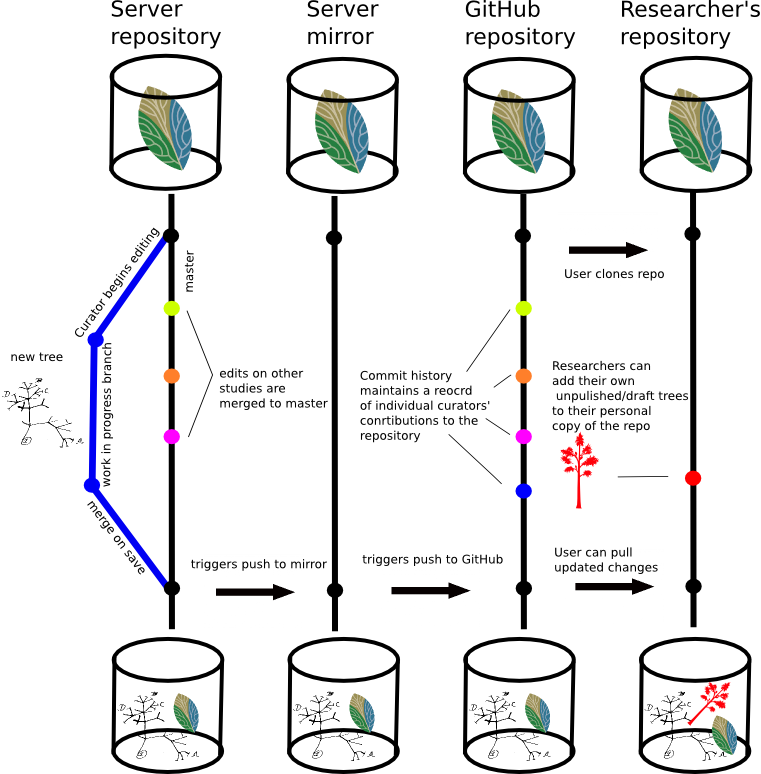
\includegraphics[scale=0.4]{workflow.png}

\section{Conclusion}
We have developed a git-based datastore for archiving and curating phylogenetic estimates of species relationships.
By incorporating curation into the data storage we have lower the activation cost of entering data into
    an archive while also allowing continued curation, allowing wither the original authors or researchers
    interested in re-using these data to improve the associated metadata.
Using git allows us to track data curation and maintain provenance, while simultaneously making it straightforward
    for researchers to maintain their own update-able copies of the database.

\section*{Acknowledgement} Thanks, Obama.\\
We thank the entire software team of the \otol project for input on design of the system;
Rick Ree and Peter Midford for implementing export features for phylografter to allow the \ps
    data store to be populated with studies from phylografter; and 
the biologists who improve the quality of data by adding and curating studies.
Jonathan ``Duke'' Leto wrote some of the code for a preliminary version of the \ps-api tool
    which served as the initial code base for the current implementation.
\paragraph{Funding\textcolon} We thank NSF AVATOL \#1208809, HITS, and an Alexander von Humboldt award to EJM for funding.

\bibliography{phylesystem}

\end{document}

\section{Useful text that we might want to reinstate}
However, making phylogenies re-usable by researchers not involved in the original analyses often requires fairly extensive curation.
The tip labels on trees often have meaning in the context of that analysis that are not easily translated across studies. 
For example, the tip labels may contain abbreviations, or lab sample codes.
Data reuse requires standardizing labels so that they are meaningful across studies.
Taxonomic name recognition services, such as ?? Plant something, or ?? taxomachine, can attempt to automatically map names to
operational taxonomic units, but this process also requires come subjective human intervention. 

By supporting contribution and curation in an open and accessible manner, we hope to provide a database with longterm utility and widespread adoption.



\section{notes}
 The current (as of May) data set
 Community contributed phylogenies

 - 6745 trees from 2914 published studies
 - 1188 trees from 991 studies partly curated 
 - 335 trees from 327 studies completely curated and included in the synthetic tree.

 The problem:
 - Large data set: Thousands of phylogenies, and always growing (hopefully!)
 - Each phylogeny requires some hand curation, often by multiple people
 - Need to be readily accessible, and editable by interested researchers
